\documentclass{beamer}

\usepackage{cmap}
\usepackage[T1,T2A]{fontenc}
\usepackage[utf8]{inputenc}
\usepackage[russian]{babel}

\mode<presentation> {
\usetheme{Madrid}
\setbeamertemplate{caption}[numbered]
}

\usepackage{graphicx} % Allows including images
\usepackage{booktabs} % Allows the use of \toprule, \midrule and \bottomrule in tables

\title[Системное программирование]{Процесс загрузки GNU/Linux}

\author{Мартынов Семён}
\institute[СПб ПУ]
{
Санкт-Петербургский политехнический университет Петра Великого\\
\medskip
\textit{semen.martynov@gmail.com}
}
\date{\today}

\begin{document}

\begin{frame}
\titlepage
\end{frame}

\begin{frame}
\frametitle{Содержание}
\tableofcontents
\end{frame}

%------------------------------------------------
\section{Этапы загрузки}
%------------------------------------------------

\begin{frame}
\frametitle{Этапы загрузки}

Процесс загрузки выполняет следующие шаги:
\begin{itemize}
\item{[ Power On => ] Reset CPU (код процессора) \\
Передача управления на 0xffff0 [cs = 0xf000, ip = 0xfff0] - BIOS SC\\
Power-on self-test (POST) POST (Power On Self Test)}
\pause
\item{Опредление устройств с собственными BIOS и их инициализация\\
Memory Test, настройка параметров устройств\\
Выбор загрузочного устройства\\
Передача управления загрузчику (Jump at 0x7c00)}
\pause
\item boot-loader (512 байт) - загружает grub
\pause
\item GRUB - загружает ядро и initramfs
\pause
\item Ядро ищет и стартует оборудование
\pause
\item initramfs (/sbin/init) готовит всё для запуска ОС
\pause
\item Change Root на настоящую систему
\pause
\item /sbin/init настоящей системы запускает программы.
\pause
\item Стартует getty или даже gdm
\end{itemize}

\end{frame}

%------------------------------------------------

\begin{frame}
\frametitle{Процесс загрузки}

\begin{figure}
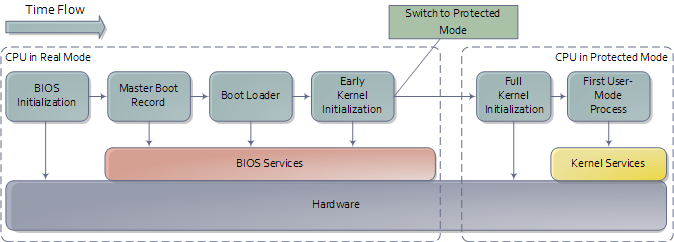
\includegraphics[scale=0.5]{res/bootProcess}
\end{figure}

\end{frame}

%------------------------------------------------
\section{Простейший boot-loader}
%------------------------------------------------

\begin{frame}
\frametitle{Простейший boot-loader}

\begin{figure}
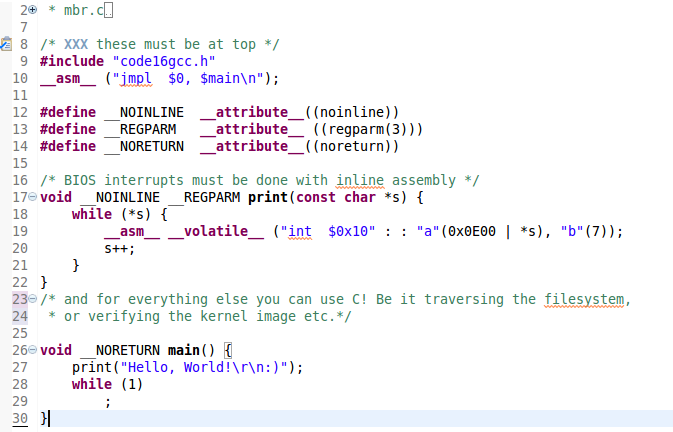
\includegraphics[scale=0.5]{res/mbrc}
\end{figure}

\end{frame}

%------------------------------------------------

\begin{frame}[fragile]
\frametitle{Простейший boot-loader: проблемы}
Код не будет работать!
\vspace{3em}
\pause

Проблемы:
\begin{itemize}
\item pеальный режим работы процессора
\item elf файл
\end{itemize}
\vspace{3em}
\pause

Решения:
\begin{itemize}
\item \begin{verbatim}__asm__(".code16gcc\n");\end{verbatim}
\item специальный шаблон линкера
\end{itemize}

\end{frame}

%------------------------------------------------

\begin{frame}
\frametitle{Шаблон линкера}

\begin{figure}
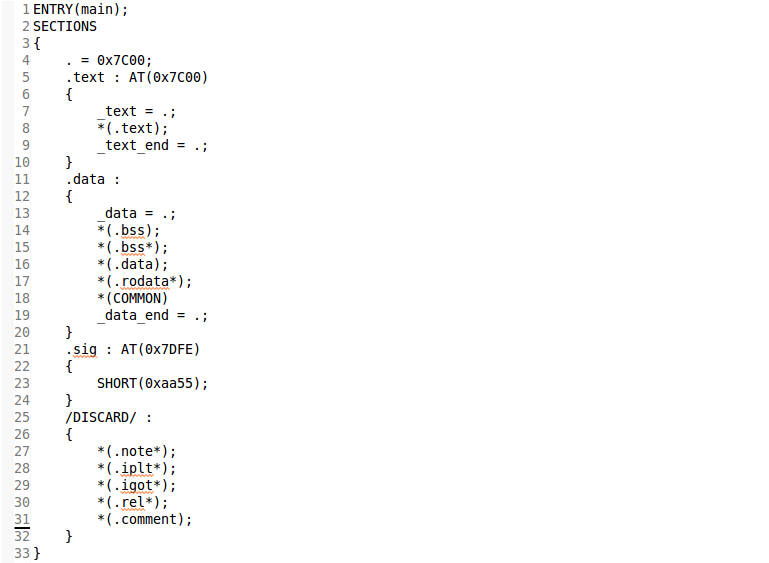
\includegraphics[scale=0.4]{res/linker}
\end{figure}

\end{frame}

%------------------------------------------------

\begin{frame}
\frametitle{Компиляция}

\begin{itemize}
\item[\$]gcc -c -g -Os -m32 -march=i686 -ffreestanding -Wall -Werror -I. -o mbr.o mbr.c
\item[\$]ld -static -melf\_i386 -Tlinker.ld -nostdlib --nmagic -o mbr.elf mbr.o
\item[\$]objcopy -O binary mbr.elf mbr.bin
\vspace{3em}
\item[\$]dd if=/dev/zero of=floppy.img bs=1024 count=1440
\item[\$]dd if=mbr.bin of=floppy.img bs=1 count=512 conv=notrunc
\vspace{3em}
\item[\$]qemu-system-i386 -fda floppy.img -boot a
\end{itemize}

\end{frame}

%------------------------------------------------

\begin{frame}
\frametitle{Тест}

\begin{figure}
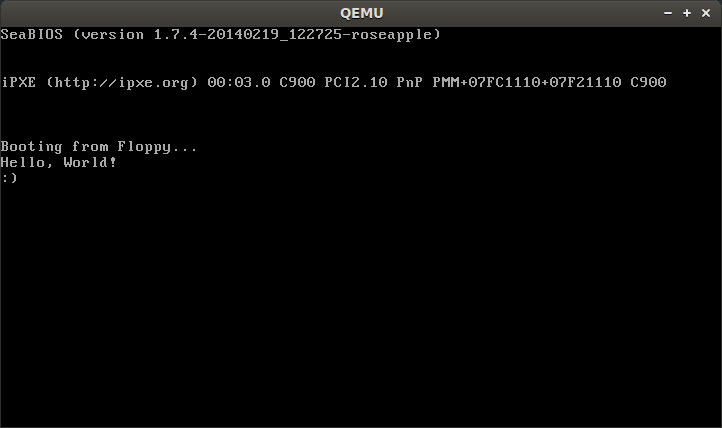
\includegraphics[scale=0.48]{res/qemu}
\end{figure}

\end{frame}

%------------------------------------------------
\section{Вопросы}
%------------------------------------------------

\begin{frame}
\begin{minipage}[t][.8\textheight]{\textwidth}
	\vspace{5em}
    {\Huge{\centerline{Вопросы?}}}

    \vfill

    Исходные коды:\\ \url{https://github.com/SemenMartynov/SPbPU_OSandComponents}
\end{minipage}
\end{frame}

%----------------------------------------------------------------------------------------

\end{document} 
